% !TeX root = ../../../main.tex
\begin{figure}[!ht]
\ChThreeFloatContents
  {ch03:fig:ite_injectable}
  { \caption{
  Distribution of Estimated Individual Treatment Effects (ITE) for different medication adherence groups: \textcolor{ChThreeForestGreen}{injectable}, \textcolor{orange}{non-injectable}, and \textcolor{purple}{not covered} at time snapshot \(\tau=3\) months. 
    Each plot's legend highlights the Average Treatment Effect (ATE) in months for the groups covered by \textcolor{ChThreeForestGreen}{injectable} medication, \textcolor{orange}{non-injectable} medication, and those \textcolor{purple}{not covered} by any medication. 
  (a)-(c): T-learner ITEs for CoxPH, DeepSurv, and Random Survival Forest. 
  (d): ITE for Causal Survival Forest.}}
  {%
    \subfigure[\footnotesize (CoxPH, T-Learner)]{\label{ch03:fig:ite_injectable_coxph}%
      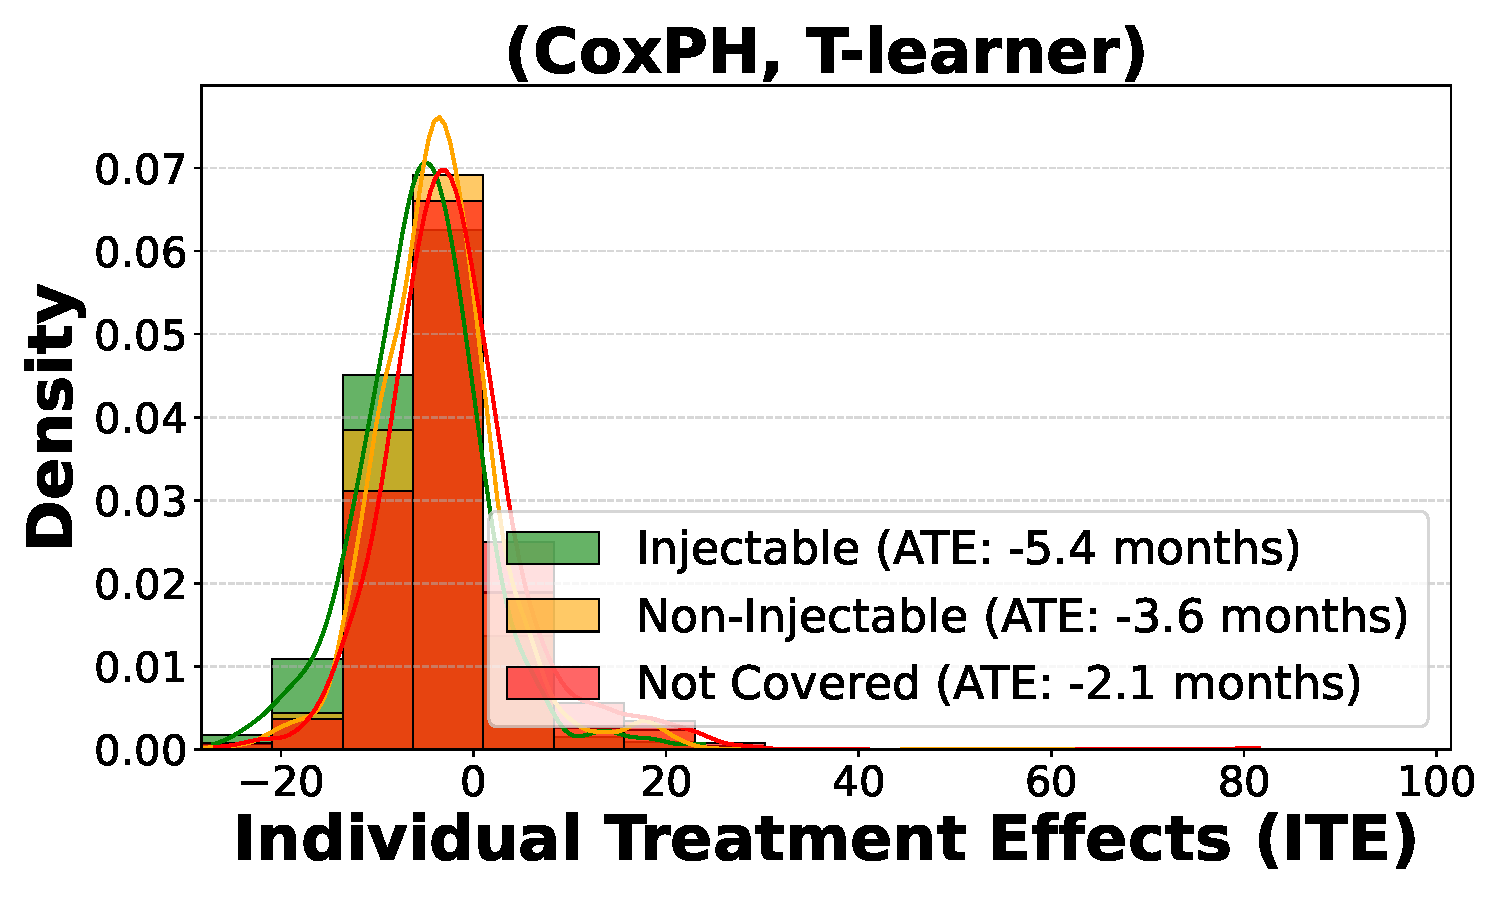
\includegraphics[width=.22\linewidth]{Chapters/chapter-03/images/ITE_injectable/ITE_CoxPH_T-learner_injectable_type.pdf}}%
    \hfill
    \subfigure[\footnotesize (DeepSurv, T-Learner)]{\label{ch03:fig:ite_injectable_deepsurv}%
      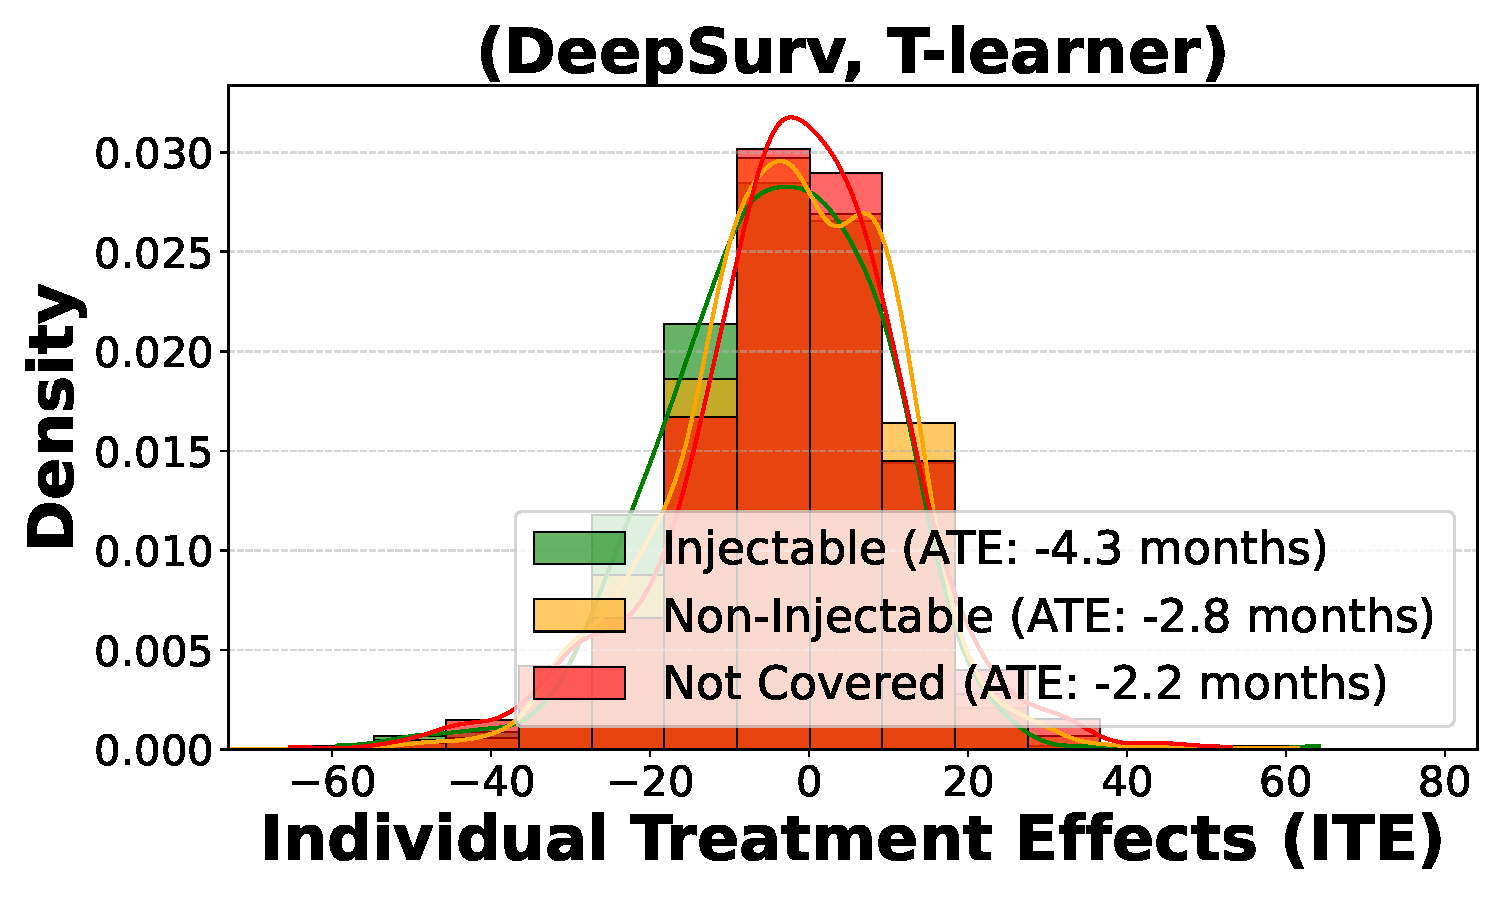
\includegraphics[width=.22\linewidth]{Chapters/chapter-03/images/ITE_injectable/ITE_DeepSurv_T-learner_injectable_type.pdf}}%
    \hfill
    \subfigure[\footnotesize (RandomSurvivalForest, T-Learner)]{\label{ch03:fig:ite_injectable_random_survival_forest}%
      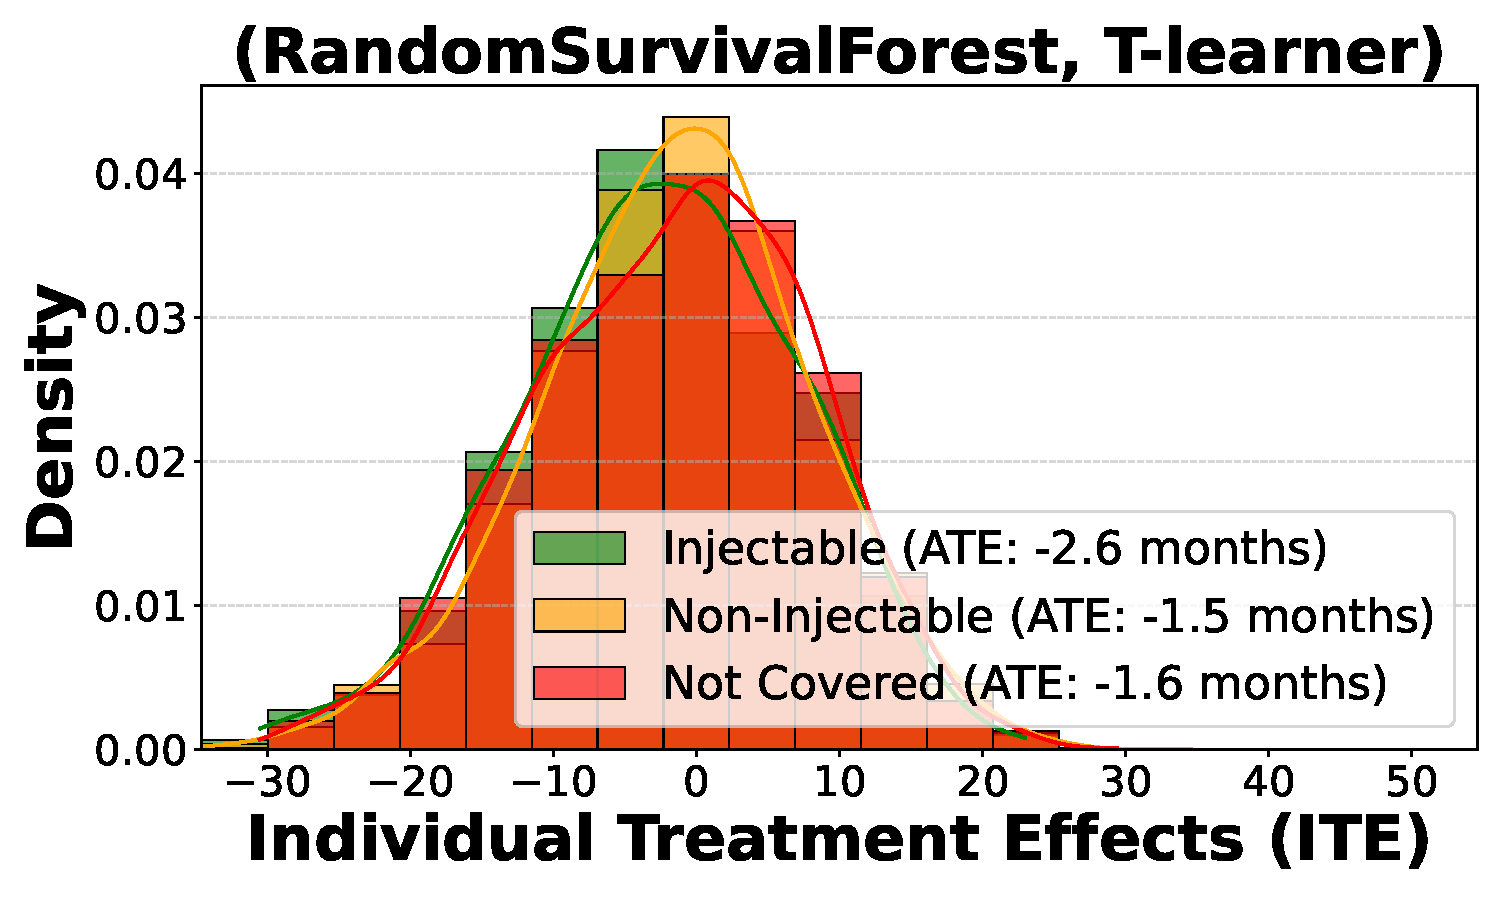
\includegraphics[width=.22\linewidth]{Chapters/chapter-03/images/ITE_injectable/ITE_RandomSurvivalForest_T-learner_injectable_type.pdf}}%
    \hfill
    \subfigure[\footnotesize CausalSurvivalForest]{\label{ch03:fig:ite_injectable_causal_survival_forest}%
      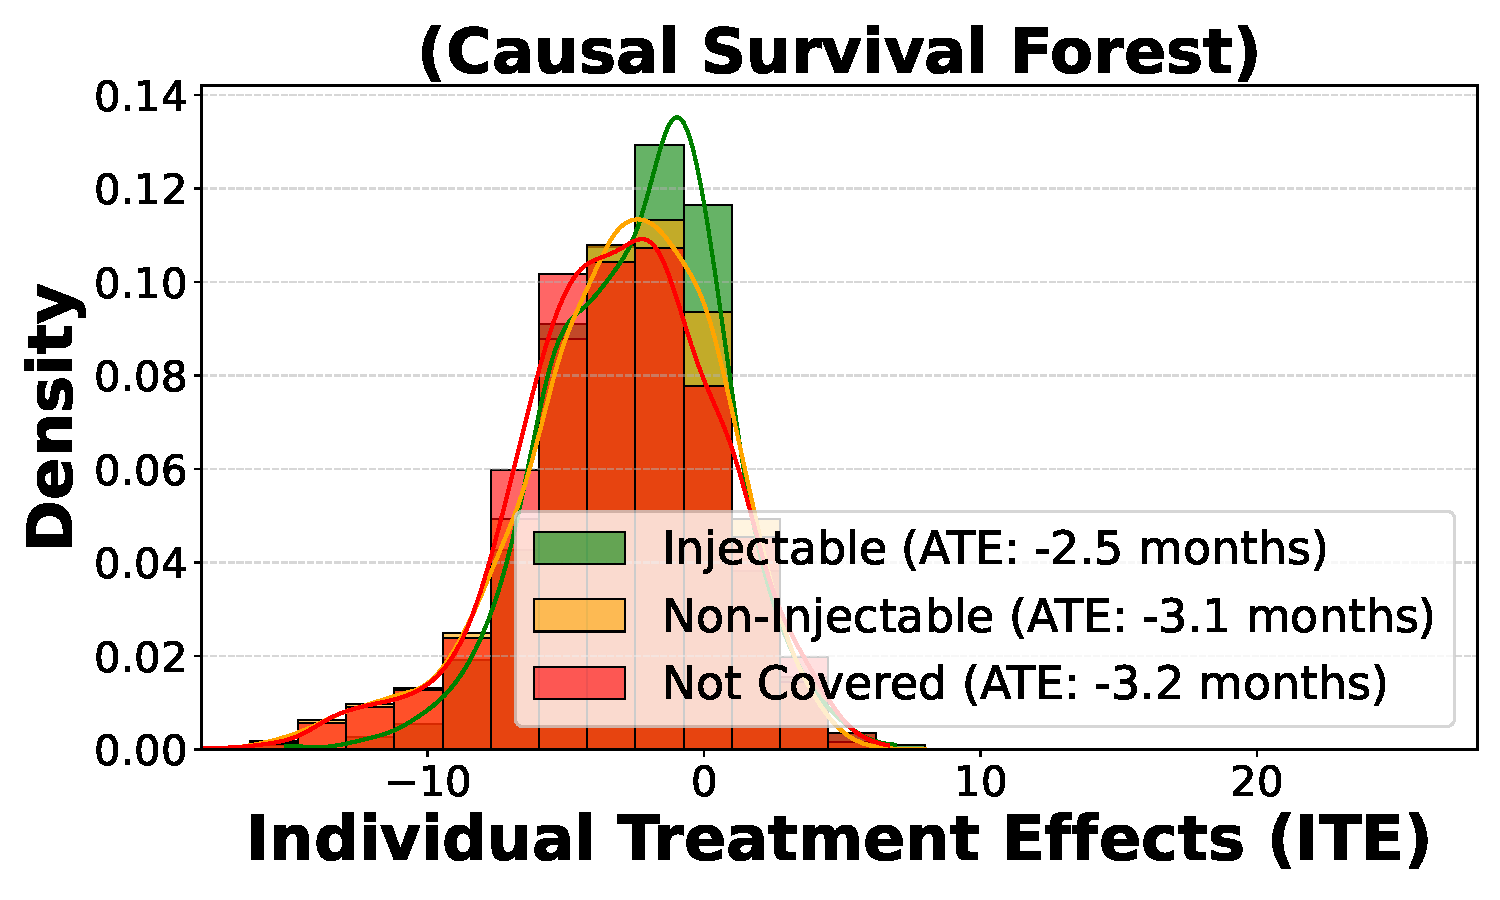
\includegraphics[width=.21\linewidth]{Chapters/chapter-03/images/ITE_injectable/ITE_CausalSurvivalForest_Causal_Survival_Forest_injectable_type.pdf}}%
  }
\end{figure}